\section{Temperature Box}

Even though previous setups used an infrared lamp~\cite{Boano2013, Hermans2013} to heat the motes directly, we chose to control mote temperature sorely using air temperature.
The mote is placed in a closed styrofoam box and the confined air is heated to the requested temperature and circulated to transfer this heat to the mote.

\subsection{Hardware}
A microcontroller evaluates temperature sensors within the box and locally controls the duty cycles of the PC fan and 150W ceramic heating element using a PID loop to achieve the requested air temperature.
The controller is equipped with a serial connection to be used to set the desired temperature and read out the actual temperature.

Additionally air temperature is displayed as a hue from blue (cold) via green (warm) to red (hot) by an RGB LED and the duty cycles of the heating element and fan are mapped to two white LEDs, to provide an immidiate heating system overview and prevent burn injuries.

The box is powered by an ATX power supply, chosen for its wide availibility and the ability to provide 12V, 5V and 3.3V at the required currents, which removes the need for additional (costly) voltage conversion.
A custom designed PCB distibutes power from the ATX connectors to two high and two medium power MOSFET switches and up to four temperature sensors, all controlled by an ATmega328p.

The PCB, heating element and fan are fastened using holders on a baseplate, which were prototyped using the PCB mill and lasercutter of the RWTH FabLab~\cite{fablab}.
The styrofoam box has the outside dimensions of $35 \times 35 \times 30$cm with a wall thickness of 5cm which results in a holding capacity of $12.5\ell$.

Picture~\ref{pic:box_hardware} shows the controller, heating element, fan and mote harness.

\subsection{Embedded Software}

The embedded software is written using the xpcc microcontroller framework~\cite{xpcc.io} and implemented as a set of asynchronous control tasks for input parsing and output formatting, temperature sensor evaluation, PID loop update and duty cycle generation.
All switching frequencies were kept as low as possible to avoid any interference with the 2.4GHz band.

\subsection{Evaluation}

The heating element has enough power to create air temperatures of up to $120\,^{\circ}\mathrm{C}$, however, a limit of $90\,^{\circ}\mathrm{C}$ is imposed during experiments, since the mote is only rated up to $85\,^{\circ}\mathrm{C}$ and the styrofoam starts to break apart.
As seen in Figure~\ref{fig:box_heating_cooling} it takes about 40 minutes to heat up to $90\,^{\circ}\mathrm{C}$ and more than 2 hours to cool back down to $30\,^{\circ}\mathrm{C}$.

During the experiments a stepping heating approach is used similar to Figure~\ref{fig:box_heating_step}.

With a room temperature of $20-25\,^{\circ}\mathrm{C}$, the minimum experiment temperature was set at $30\,^{\circ}\mathrm{C}$ so that it can be reached within reasonable time.
The boxes can be retrofitted with an active piezoelectric cooling element and a fan by connceting them to the two unused MOSFET switches on the controller and updating the software.

\begin{figure}[t]
	\centering
    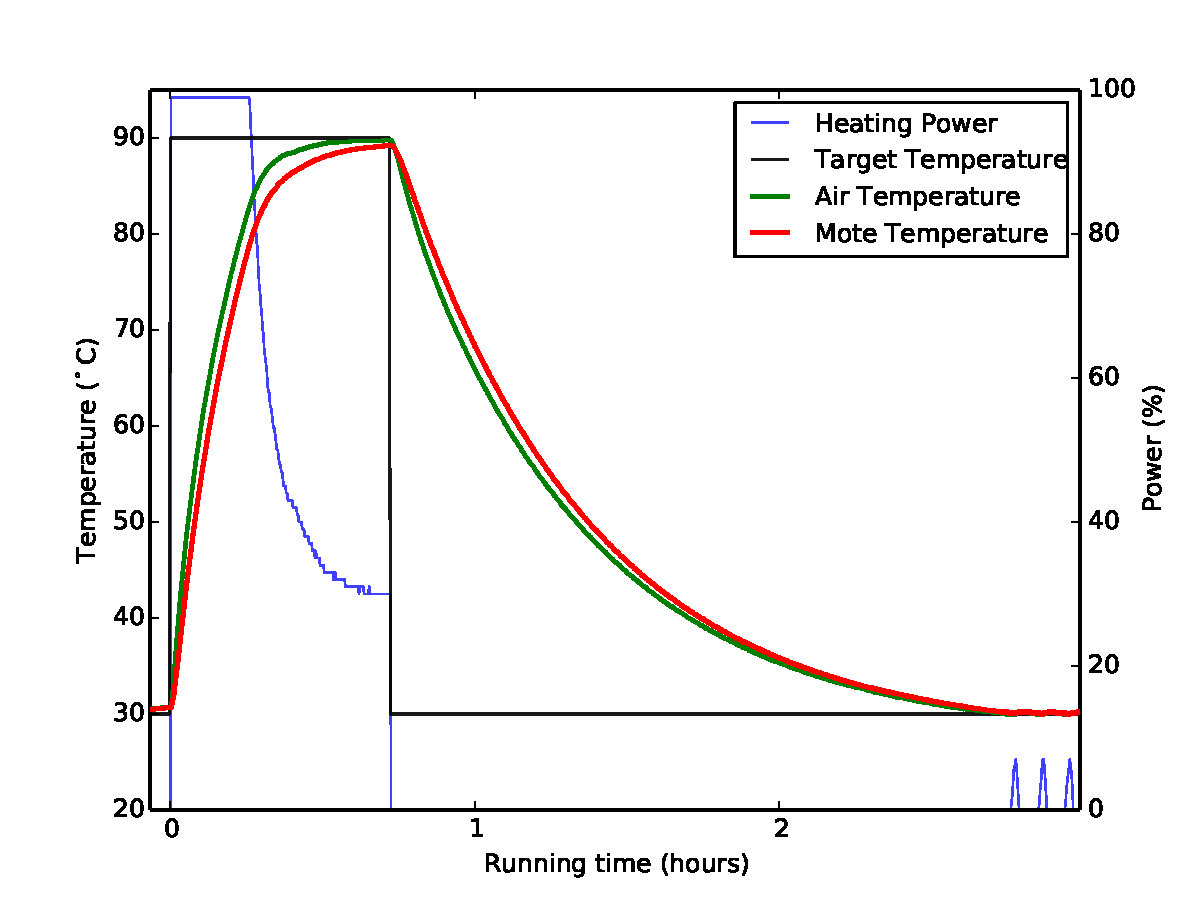
\includegraphics[width=1\columnwidth]{figures/box_heating_cooling}
	\caption{Temperature box heating up to $90\,^{\circ}\mathrm{C}$, then cooling back down to $30\,^{\circ}\mathrm{C}$.}
    \label{fig:box_heating_cooling}
\end{figure}

\begin{figure}[t]
	\centering
    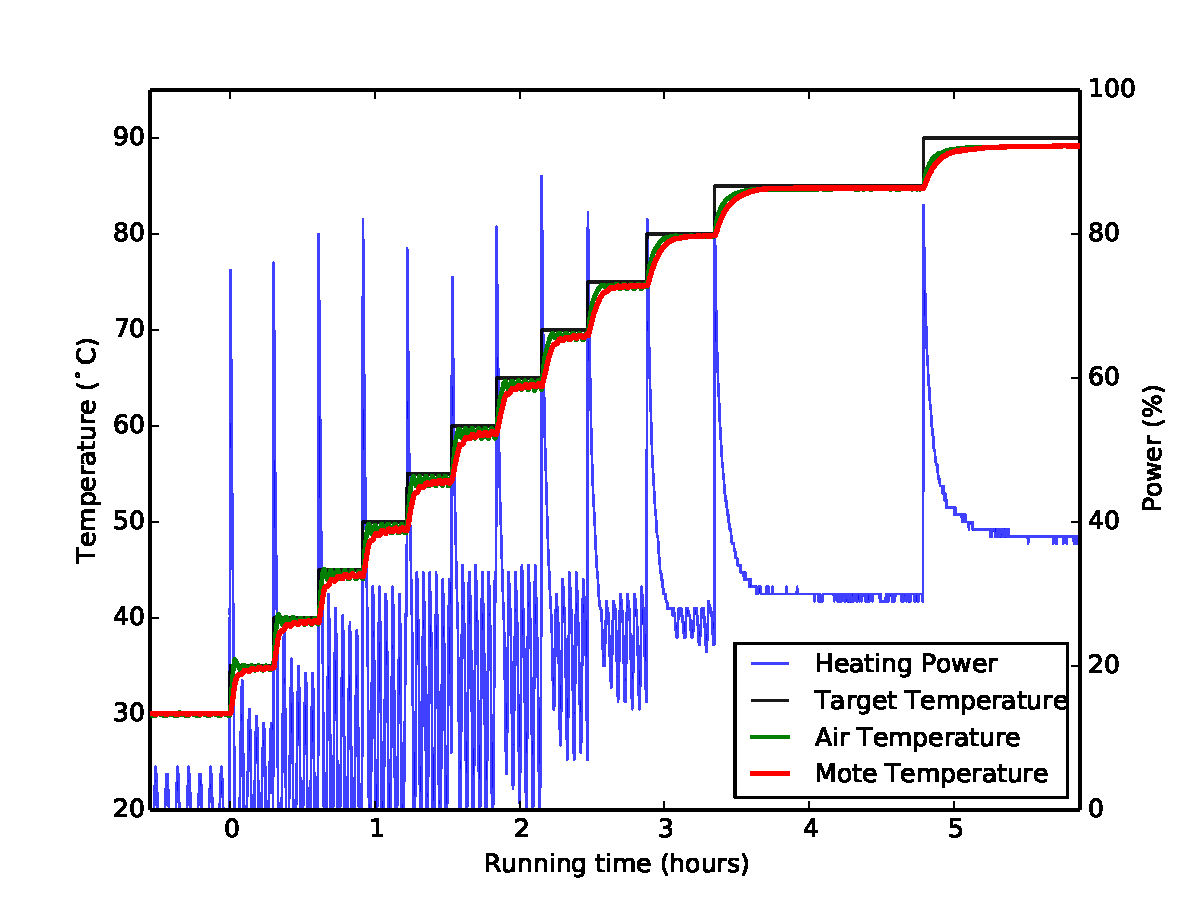
\includegraphics[width=1\columnwidth]{figures/box_heating_step}
	\caption{Typical experiment setup with temperature increases in steps of $5\,^{\circ}\mathrm{C}$.}
    \label{fig:box_heating_step}
\end{figure} 